\subsection{Detailed results on larger cohort with only cognitive scores}
We also applied our method to a larger cohort consisting of approximately 1500 subjects with varying temporal measurements on the battery of cognitive tests. Each individual had approximately 3 visits worth of data, and so our total number of measurements was approximately $n = 4000$. In addition to the groupings used above, we were able to use an algorithmic cognitive impairment (ACI) measure to further evaluate the model against a factor which is known to be group-separating. Below are the tabulated feature sets identified by our model for each of the group separations described in the main thesis. In this case to increase interpretability of the results we limited our search to groups of 3-6 features.

When grouped by genotype, the most indicative subset as shown in Table \ref{fig:coggenotype}. These tests are most closely associated with memory, and we see that no tests of executive function or spatial ability (Trail-Making or Clock Drawing) were included.

In addition to an algorithmic measure of impairment, a conference of expert clinicians and researchers have given each individual a clinical impairment diagnosis for each time they underwent the cognitive battery. Using this as a group separator, we found a large number of overlapping subsets that displayed significant group difference at the $p = 0.05$ level. These are shown in Table \ref{fig:cogcc}. Trail-Making Test Parts A and B appeared in all identified subsets.

\begin{table}
	\centering
	\begin{tabular}{p{0.8cm}p{5.5cm}p{6cm}}
		\toprule
		\multicolumn{3}{c}{\textbf{Algorithmic Cognitive Impairment}}\\ \midrule \midrule
		Set 1 & Boston Naming Test Total Score & RAVLT Learning Trial A1 Raw Score \\ 
		 & RAVLT Learning Trial A6 Raw Score &  \\ \bottomrule
		\bottomrule
	\end{tabular}
	\caption{Group Difference Localization Across Algorithmic Impairment}
\end{table}

\begin{table}
	\centering
	\begin{tabular}{p{0.8cm}p{5.5cm}p{6cm}}
		\toprule
		\multicolumn{3}{c}{\textbf{Genotype: ApoE4}}\\ \midrule \midrule
		Set 1 & WAIS-III Digit Span Backward Raw Score & RAVLT Learning Trial A3 Raw Score \\
		& RAVLT Learning Trial A4 Raw Score & RAVLT Learning Trial A5 Raw Score \\
		\bottomrule
		\bottomrule
	\end{tabular}
	\caption{Group Difference Localization Across ApoE4 Genotype}
	\label{fig:coggenotype}
\end{table}

\begin{table}
	\centering
	\begin{tabular}{p{5.5cm}p{6cm}}
		\toprule
		\multicolumn{2}{c}{\textbf{Expert Consensus Measure}}\\ \midrule \midrule
		WAIS-3 Letter-Number Sequencing Raw Score &
		Boston Naming Test Total Score \\
		RAVLT Learning Trial A2 Raw Score &
		RAVLT Learning Trial A3 Raw Score \\
		RAVLT Learning Trial A4 Raw Score &
		RAVLT Learning Trial A5 Raw Score \\
		RAVLT Learning Trial A6 Raw Score &
		RAVLT Delayed Recall Raw Score \\
		Trail-Making Test Part A &
		Trail-Making Test Part B \\
		Clock Drawing Test Score &
		Center for Epidemiologic Studies Depression Scale Score \\
		\bottomrule
		\bottomrule
	\end{tabular}
	\caption{Group Difference Localization Across Expert Clinical Diagnosis}
	\label{fig:cogcc}
\end{table}

\begin{figure}
\centering
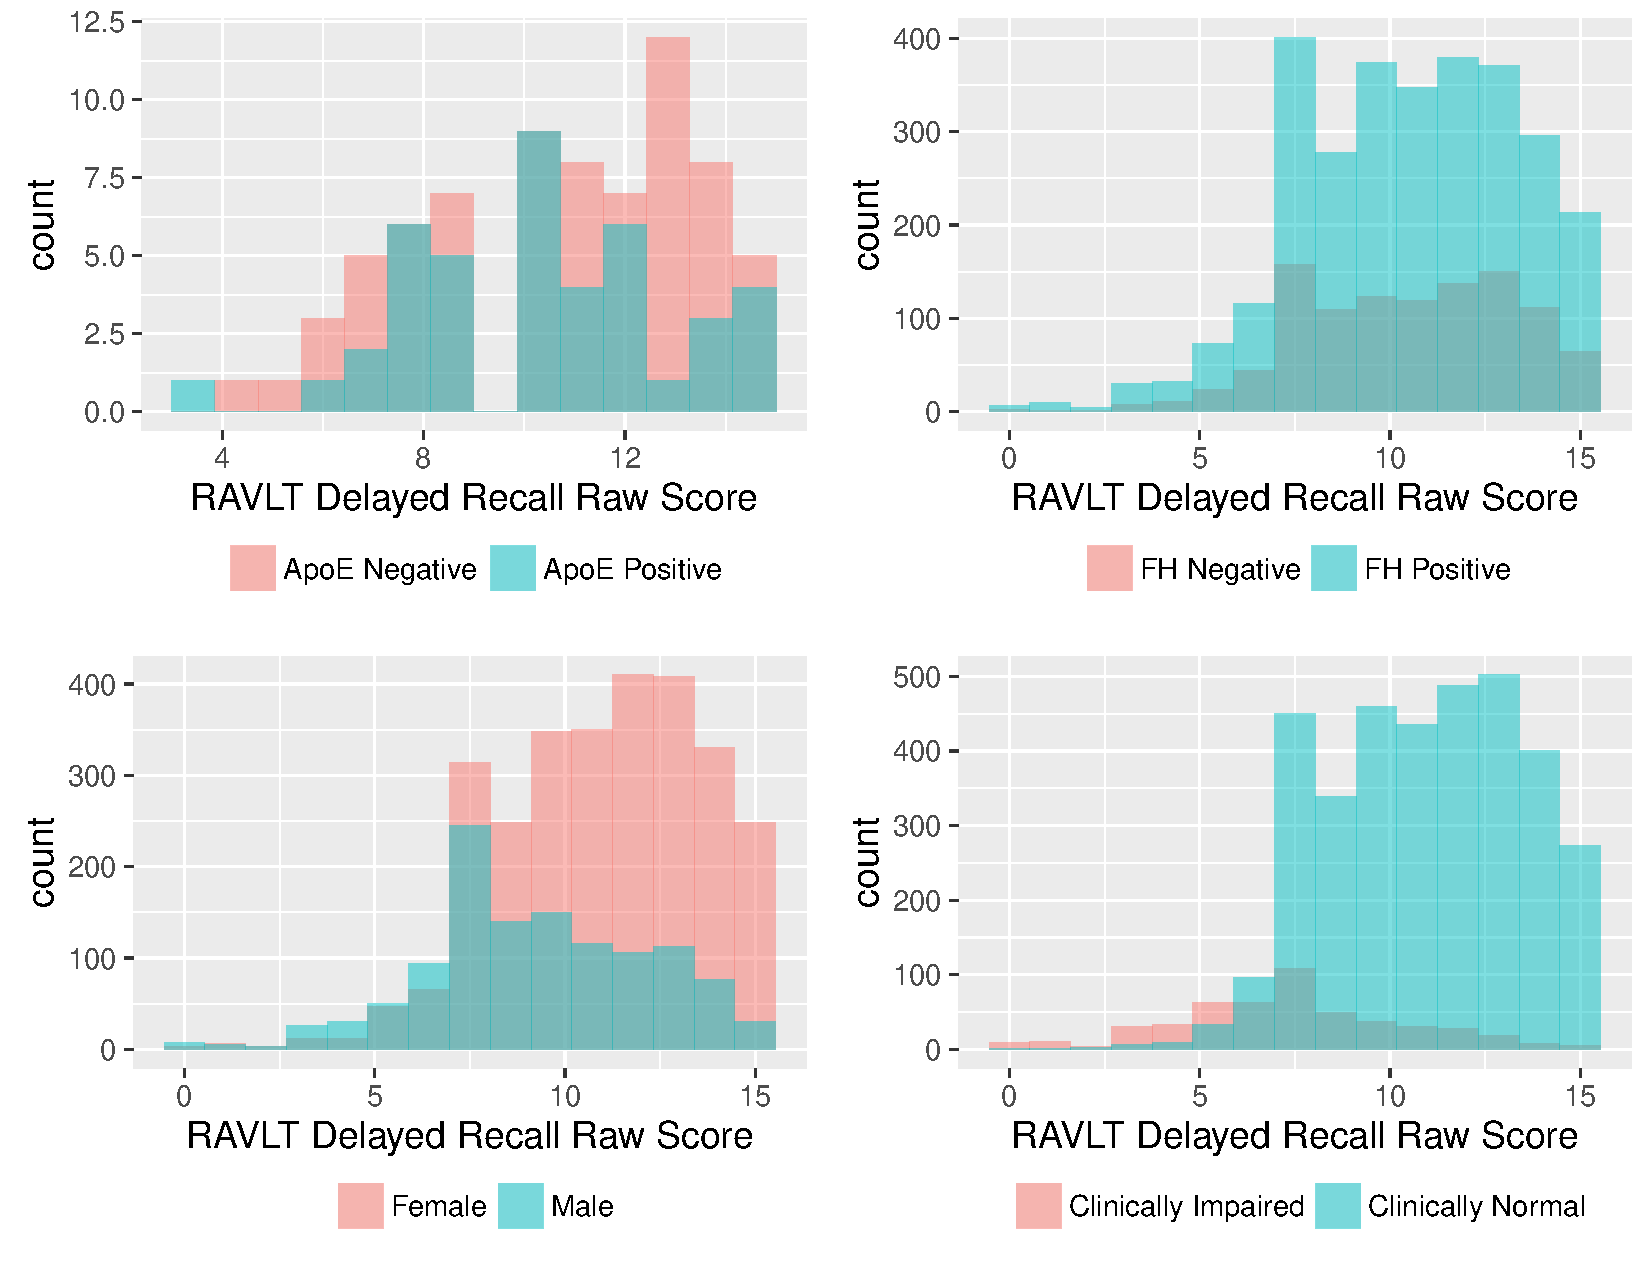
\includegraphics[width=\textwidth]{3_covtraj/figs/DRRAWHists_cogonly.pdf}
\caption[Delayed Recall Histograms]{Histograms of the Delayed Recall Scores for all time points for the $\sim 4000$ individual measurements across different group separations. We note in particular that the results found from the genotype separation above would have been hard to identify since given the distributions are extremely overlapping (top left) for this particular separation.}
\end{figure}